\chapter{Data Collection and Fuzzy Test Generation for Auto Pilots}\label{chapter:fuzz_tester}
\section{Introduction}
Model inference techniques are generally grouped into static and dynamic analysis categories. 
Static approaches use the code as their input data. They are able to gather all the required information such as function call graphs for example from the source code itself without a need to run the software.
A typical dynamic model inference pipeline, on the other hand, starts with running existing tests in the software to collect required data. \cite{Papadopoulos2015} 
The data that is generated in software run time is quite varied; It can range from the logs, to function calls, to network packets, to syscalls, and so forth. There are several aspects to be considered for this matter: what kind of data is needed, how are they going to be collected, what kind of model we are looking to have, and how are they going to be used in model inference. 

Walkinshaw et al. for example, \cite{walkinshaw2016inferring} sought to create state models as extended finite state machines. Their approach requires two collections of ordered events to work, a collection of positive examples which are events generated during a successful execution of the software as well as a set of negative examples. Each event there, is a function call; the log contains the list of functions that were called along with their parameters. 
In \cite{howar2012inferring} the events are high level actions such as `user registered` and `user logged in'. It also seeks to generate state models.
In Synoptic \cite{schneider2010synoptic} the communications in a distributed system is being modeled as an automata and the events are the logs generated by its components.


In this study the goal is to infer a state model of the system under study as a black-box without access to its source code. Therefore I am limited to observing the inputs and outputs of the system. Another piece of information that is often overlooked is time. In this study time is taken into consideration as well. I capture all the inputs and output values of the system in regular intervals. Since they are all numeric, they make a multivariate time series that I use to generate time-aware state models. 


A common theme in almost all model inference algorithms developed in the past two decades is that they use the data collected as the system functions in the wild. They either run existing test cases or instrument and inspect the system being used in production. 
This is to have a diverse collection of data that is also meaningful and representative of the actual system behaviour in common use cases.

Depending on the system under study and the type of data required, this might be an excellent way of collecting the data or might be infeasible for scalability reasons for example. That is what I encountered earlier while applying white-box model inference approaches to the industry partner's code base. The results are published in an ICPC 2019 paper \cite{mashhadi2019empirical}; to summarize that paper, the state of the art white box model inference algorithms suffer from not being scalable to be used in industry as is.
%In this study in particular there is an amalgam of both ends of the spectrum. 
As mentioned earlier, it is done on two auto pilot systems, Micro Pilot and Paparazzi. \cite{hattenberger2014using}
Although they both are highly capable and widely used drone auto pilots, their implementations are quite different which makes data collection phase quite different too.

\section{Data Collection Process}
In this section more details on how data was collected from each system will be presented. 

\subsection{MicroPilot AutoPilot}

Since a detailed overview of the data collection is discussed later in the next chapter, more specifically section~\ref{sec:mp_data_collection_process}, in this section I will only cover the related technical details about this process in MicroPilot. That is just to prevent restating what is already covered in the manuscript.

\subsubsection{Instrumentation}
Control decisions in this software are made in a 5Hz loop, it means that every 200ms all the sensor inputs are read and based on the current state of the aircraft and the system's goal at the moment (e.g. maintaining a constant speed) decisions will be made and output is generated. Considering this, the best way to capture those data is in the end of each iteration of this loop. I inserted instrumentation code there, to log input and output values at the exact spot where they are updated. 
Please note that although it is more convenient to capture the values in this way, it does not give us any special advantage or insight that breaks the black-box condition. In other words, the exact same data could be collected from the compiled binaries without any access to the internals, just with extra steps. Inputs and outputs, after all, are the very least thing available in both black-box and white-box settings.

\subsubsection{Test Scenarios}\label{sec:mp_test_scenarios}
MicroPilot has a repository of more than 900 system tests which can be run in a realistic simulator. The auto pilot can be used in SWIL and HWIL modes \cite{melmoth2019true}, which stand for software in the loop and hardware in the loop respectively. We used SWIL mode as it provides what we need without any of the overheads associated with HWIL mode. 

\subsection{Paparazzi}\label{sec:paparazzi_data_collection}

\subsubsection{Instrumentation}
Paparazzi provides a rich and flexible API that can be configured to record several different parameters in flight. The aircraft periodically sends data back to the ground station over a wireless link using a protocol called Paparazzi link. Paparazzi link is built over Ivy, a message bus protocol that uses UDP. 
In Paparazzi's architecture a process called `link' interfaces the wireless link to the aircraft to the computer's network; on one side are the Paparazzi link messages that come and go as UDP datagrams and on its other side is the (often wireless\footnote{A wired connection is used in HWIL test mode as well as some scenarios where the AutoPilot equipment is used in a autonomous submarine rather than an autonomous unmanned aircraft.}) connection to the aircraft.
In simulations, the modem and wireless communications are no longer needed, instead the auto pilot runs as a separate process and mimics a wireless channel over the local network. (See Figure~\ref{fig:paparazzi_comm_agents})

\begin{figure}
    \centering
    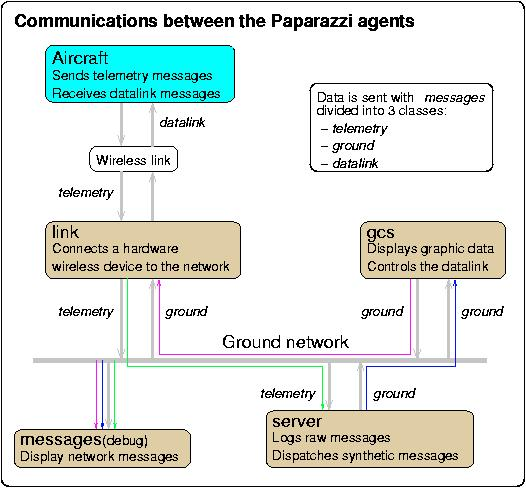
\includegraphics[width=\columnwidth]{4_files/Pprz_communication_agents.jpg}
    \caption{High level overview of communication links architecture in Paparazzi \cite{hattenberger2014using}}
    \label{fig:paparazzi_comm_agents}
\end{figure}

Paparazzi comes with a multitude of small tools that could do most of what I needed in terms of instrumentation. There is a remote logger and a log player which are quite close to the instrumentation tool I need, however upon trying them in action, I figured that they cannot record some of the information that I need. Therefore, I developed a custom flight data recorder tool. 

\subsubsection{Test Scenarios}
Unlike MicroPilot that had a quite a number of system tests (in addition to other types of tests such as unit tests which I did not use), Paparazzi comes with only unit tests. As it is an open source software under GPL licence it comes with no warranty and also does not need certain certifications and approvals that commercial systems require, therefore incentives to have such tests are lower. 
Although it is a reliable and widely used auto pilot, it owes that reliability more to its widespread use in action (by many researchers and enthusiasts) rather than automated tests that verify its behaviour.
In this situation, where many eyes are watching over the code, bugs are discovered and patched quickly. However, to the best of my knowledge they are not recorded as system tests that verify the bugs are properly patched and detect regressions in the future.

To fill the void, I created a tool that can automatically generate valid and meaningful automated system tests for Paparazzi, run them automatically, and integrate with the flight data recorder tool to generate the data set for downstream tasks. It is called Pprz Tester and the source code, version history, project planning data (bugs, enhancements, tasks and issues, etc), and the documentations are available on GitHub at \url{https://github.com/MJafarMashhadi/pprz_tester}. 

In addition to that, I needed to patch some parts of Paparazzi to make the logging and testing more similar to MicroPilot, for example increase telemetry reporting rate from 2Hz to 5Hz. A list of these patches including the reason why that change was necessary or beneficial and the exact lines of code that need to be changed is available in the project wiki at \url{https://github.com/MJafarMashhadi/pprz_tester/wiki/Paparazzi-Patches}.

Aside from the patches, I found some bugs, missing features, missing documentations, and bad smells in the code that needed to be fixed. I contributed new code and documentation to the Paparazzi project to address these issues. The contributions were useful, up to the standards, and welcome in the project; they are included in the latest release\footnote{as of August 1st, 2020} of Paparazzi auto pilot: version 5.16.

\section{The Testing and Data Processing Tool Set}
I implemented the pipeline of generating tests, running them, and aggregating flight logs in an integrated tool with three components, one for each stage. In the following sections I will explain these components and their role in the system. I also explain how event-driven programming paradigm was implemented here both to decrease coupling and to make it more resilient to unexpected or buggy behaviour. It is necessary for two reasons: 1. as a testing tool, it is \textit{expected} to encounter bugs in software under test and should be resilient to them 2. the message passing design of Paparazzi architecture, in addition to its ability to support multiple aircraft in flight at the same time left me with no choice but to use an event-driven design.


\subsection{Flight Data Recorder}
Although Paparazzi comes with a logging feature in its `server' component (Figure~\ref{fig:paparazzi_comm_agents}), it only logs a subset of required data. Furthermore, the data comes in separate messages with different frequencies; for example speed updates are sent in \verb|AIRSPEED| message once a second, orientation updates and engine rpm are reported in \verb|ATTITUDE| and \verb|ENGINE_STATUS| messages respectively which are dispatched every 200 milliseconds, while servo outputs are only sent once every 5 seconds. All these data need to be aggregated and aligned. Please refer to the Table~\ref{tab:pprz_messages} in \hyperref[appendixa]{Appendix~A} for a full list of messages used.

The most flexible option with the least overhead is to have an independent module that understands Paparazzi link, captures these messages and does data aggregation and logging in real-time. So I created a flight data recorder to collect all the required data from telemetry messages.

In the beginning the instance of ``AircraftManager'' singleton class starts with listening for \verb|NEW_AIRCRAFT| messages. This message type notifies this class when new aircraft come online in the simulation. Then it sends a \verb|AIRCRAFTS_REQ| request message to server to get a list of currently online aircraft. The response to both of these messages are processed in the same way: The aircraft unique ID will be checked against the hash table of known aircraft, if it is a new one an ``Aircraft'' instance will be created and added to the hash table. (See the class diagram in Figure~\ref{fig:fdr_class_diagram} in \hyperref[appendixa]{Appendix~A})

Each ``Aircraft'' object in the makes a number of requests back and forth with other components in the system (server, data link, and the auto pilot process) to gather required information about that aircraft, including its flight plan. This class along with ``Aircraft Parameters'' and ``Aircraft Commands'' provide a unified programmatic API for monitoring and controlling the aircraft. 

I implemented observer pattern \cite{gamma1995design} in ``Aircraft Parameters'' to enable other components (such as flight data recorder and automated test executor) to listen for changes in the aircraft state and respond accordingly in an event-driven manner. 
After creation of an ``Aircraft'' object, as a part of its initialization, several observers are created and attached to it. A ``Record Flight'' instance is one of them. It observes new \verb|FLIGHT_PARAM| messages as well as changes in `throttle', `flight time', and `commands.values' parameters. This class stores and aligns these parameters in a pandas data frame which is stored on disk periodically. The data can be stored in a human-readable CSV file or as a compressed HD5 binary. Some data normalization and unit conversions (such as meters to feet) also happen before saving in order to make the generated data similar to MicroPilot's.

Supplementary UML diagrams are provided in \hyperref[appendixa]{Appendix~A}.


\subsection{Automated Test Executor}
The test executor takes the control of the aircraft by running prefabricated test scenarios. While the low leve control of the aircraft is done by the auto-pilot software (the system under test), it needs high level commands such as `climb to 200ft'. Automated test executor does that, using hand crafted test scenarios or the ones generated by the test generator component.

Tests scenarios are defined as subclasses of \verb|PlanBase| class. Each plan needs to override a method that returns an iterable of plan items which should be executed one by one. 
\begin{lstlisting}[language=Python, basicstyle=\linespread{0.1}]
class ExamplePlan(PlanBase):
  def get_items(self, **kwargs):
    block_name = kwargs.pop('block_name')
    circles = int(kwargs.pop('circles'))
    return [items.JumpToBlock(block_name),
      items.WaitForCircles(n_circles=circles)]
\end{lstlisting}
The above plan for example, takes a block name and a number of circles as its parameter and executes the two items in succession. An example of running this plan can be like the command below:
\begin{lstlisting}[language=bash]
$ run_test.py ExampleAircraft ExamplePlan\ 
    -Dblock_name='loiter' -Dcircles=2
\end{lstlisting}
Using this parameters is analogous to test parameterization in mature unit testing frameworks (such as pytest). It allows similar test plans that are only different in some parameters to be consolidated in one test case.
Using parameters also improves the reproducibility of test scenarios while improving its flexibility. Test scenarios (plans) do not need to include commands for waiting for aircraft to take off and land, the testing tool automatically wraps it with appropriate initialization code.

The core test plan runner is implemented as an observer class that listens for multiple messages and parameters to get notified about changes in the aircraft's state (See Figure~\ref{fig:flight_plan_executor_class_diagram} in \hyperref[appendixa]{Appendix~A}). It iterates over the flight plan items and calls their \verb|match| method to decide whether that item should be executed. Whenever a match is found the item will be executed and the iterator will move to the next test plan item. Consult Figure~\ref{fig:flight_plan_items_class_diagram} in \hyperref[appendixa]{Appendix~A} for a class diagram of all flight plan items.

Test plans should be importable from \verb|pprz_tester.generated_plans| module. The structure is simple and clearly defined so that they can easily be handcrafted (like the example above) or generated using the test generator component.

The test runner is tailored specifically for Paparazzi in several ways:
\begin{enumerate}
    \item % First, 
As mentioned before, it takes care of aircraft initialization, take off, and landing
    \item %Second, 
It uses standard Paparazzi environment variables such as \verb|$PAPARAZZI_HOME|.\footnote{If it is not set, the user can use \texttt{-p /path/to/paprazzi} command line argument to set this value, and if that is not set too, a default value will be used.} 
    \item %Third, 
It can build the auto pilot if \verb|--build| argument is set so the user does not have to build it manually in Paprazzi center. 

    \item %Fourth, 
If \verb|--gcs| argument is set, the ground control station window will be opened (See Figure~\ref{fig:paparazzi_gcs}). It provides a real-time map that visualizes the aircraft path, waypoint locations, wind direction and velocity, and several other parameters of the aircraft such as their airspeed and altitude. 
    \item %And last, 
\verb|--no-sim| argument tells tester to not launch the simulator. Its use case can be when a physical auto pilot is being used (similar to MicroPilot's HWIL mode), or when for any reason the user chooses to run the simulator manually. 
\end{enumerate}

\begin{figure}
    \centering
    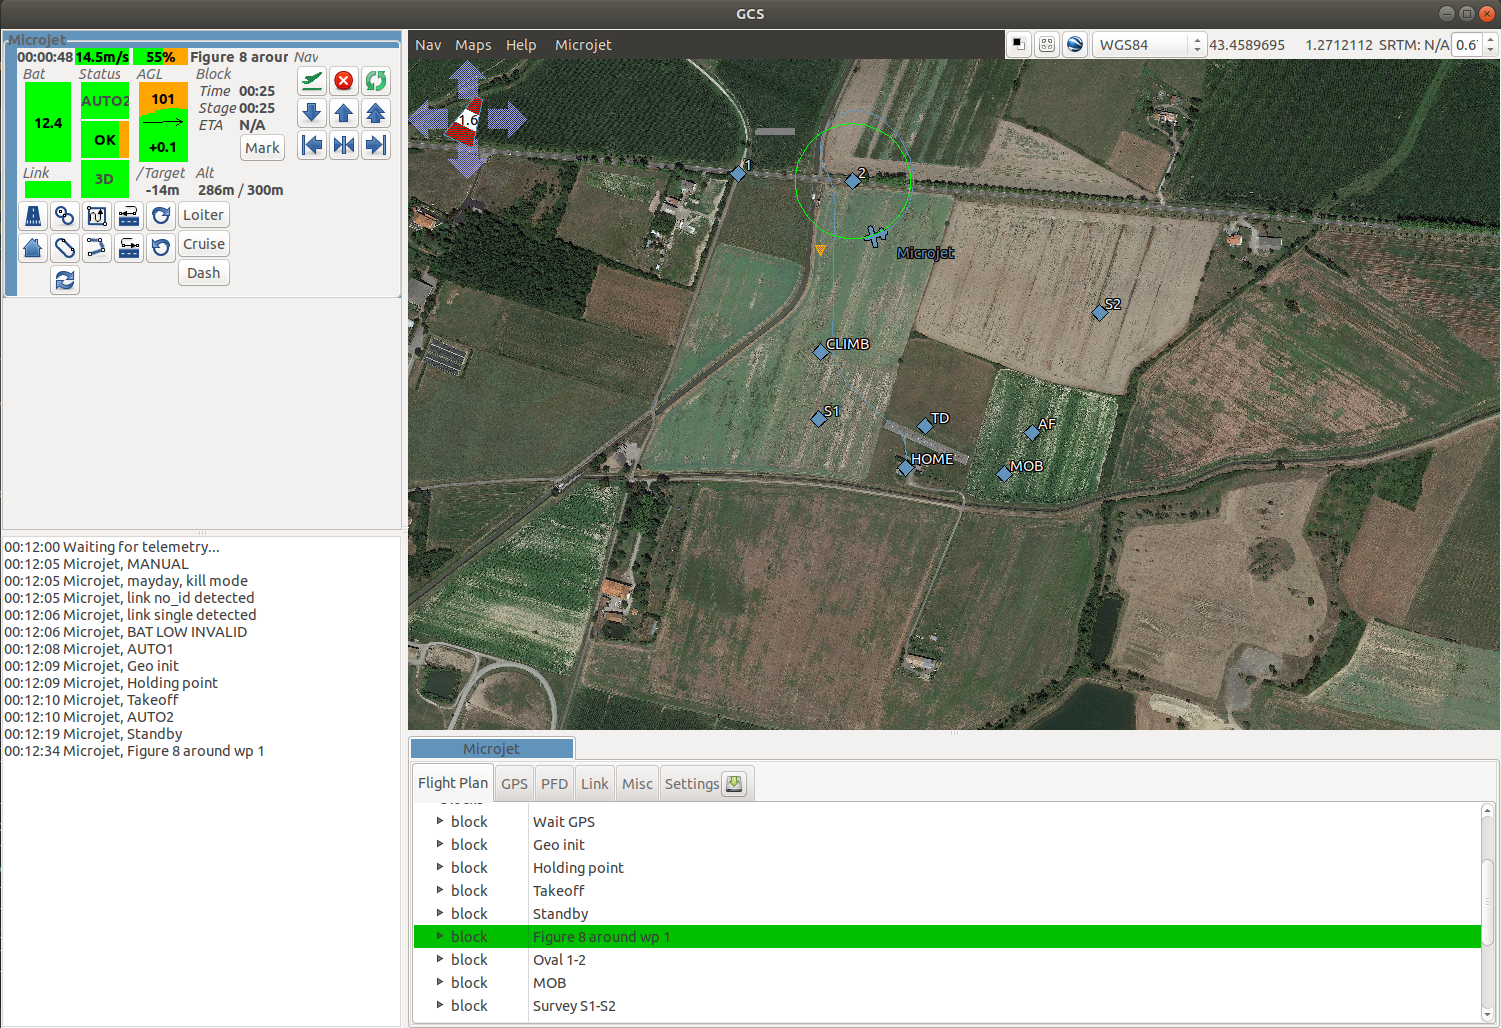
\includegraphics[width=\textwidth]{4_files/GCS.png}
    \caption{A snapshot of ground control station software (GCS), visualizing the map, waypoints (blue diamonds), the aircraft, its flight history (blue), the intended flight path (green), as well as its state (bottom in green) and some telemetry data (top left). The plan that it is following is one of the automatically generated test scenarios.}
    \label{fig:paparazzi_gcs}
\end{figure}

Test runner can move waypoints as well. The user can fix any number of waypoints at specified locations, providing their latitude longitude and altitudes. It can also randomize their location inside a cube. Boundaries of that cube (i.e. east-west, north-south, and floor-ceiling) are customizable through provided command line arguments.

The comprehensive list of command line arguments is included in Table~\ref{tab:test_runner_commandline_args} in \hyperref[appendixa]{Appendix~A}.


\subsection{Automated Test Generator}
The test generator component is a fuzz test generator specifically designed for Paparazzi. An auto pilot has plenty of parameters to change. Many of them need to remain unchanged. For example, changing aerodynamic and physical parameters of an air frame will make it behave incorrectly or even crash. A naïve algorithm might be tempted to only change these parameters to optimize a metric of ``bug''s per test. To comply with the constraints in input format and range and optimize test scenario diversity without having to have thousands of tests, I opted for developing a specialized automated test generator. 

This test generator is completely compatible with Paparazzi and designed with specific needs of an auto pilot in mind. It begins with loading and parsing the one fixed wing flight plan that comes with Paparazzi. It defines multiple actions (control blocks) available to a fixed wing aircraft. Two important components in the flight plan that are used are the waypoint names and locations, and available blocks. A test scenario is generated by taking the initial flight plan and fuzzing three parameters about it:
\begin{enumerate}
    \item Waypoint locations
    \item Sequence of actions 
    \item Action timing
\end{enumerate}

The test generator can be configured to fuzz all or some of them. I generated 31 tests with fuzzing the last two. Please note that the sequence of actions can have any length between 1 and the number of possible actions (5, in my case). Also for each sequence, $n!$ different permutations can be made that will result in very different outcomes. That makes the number of tests, $5!\times1+4!\times5+3!\times10+2!\times10+1!\times5=325$. Also note that these generated tests are made of unique blocks, in other words, a test scenario does not contain plans like ``Do A then B then A again'' while these plans are perfectly valid. In case one wants to have such plans they can write test plans manually.

The output is a python module that contains a subclass of \verb|PlanBase|, as expected by the automated test executor. These two work together seamlessly and the user can just use them in a plug-and-play manner without touching the code. Though, the generated code is designed to be effortlessly understandable and easily editable it even incorporates some auto-generated comments in the code.

The full table of command line arguments that test generator accepts is presented in Table~\ref{tab:test_generator_commandline_args} in \hyperref[appendixa]{Appendix~A}. To provide an example, the following command generates tests of length (number of actions) 2 for `Microjet' aircraft and writes it to the file \verb|l2.py| in the specified directory. It fuzzes the location (latitude, longitude, and altitude) of waypoint `S2' in the default cube, just overriding the altitude bounds in 200 to 220 meters, while the coordinates of `S1' are fixed. The initialization and landing stages which must be excluded from the test scenario are also specified. 
\begin{lstlisting}[language=bash]
gen_test.py --exclude "Wait GPS" "Geo init" "Holding 
point" Takeoff Standby "Land Right AF-TD" "Land Left 
AF-TD" land final flare --fuzz-wps S2 \
--wp-fuzz-bounds-alt 200 220 -w S1 43.4659053 1.27 300 \
--length 2 Microjet pprz_tester/generated_plans/l2.py
\end{lstlisting}
Some of the available actions and all the waypoints in this flight plan can be seen in Figure~\ref{fig:paparazzi_gcs}.